\documentclass[12pt]{article}
\usepackage[a4paper, margin=.30in]{geometry}
\usepackage{graphicx ,
            wrapfig,
            xcolor, 
            enumerate,
            amsmath,fontenc, mhchem,makecell, mhchem,tcolorbox,tikz,fancyhdr
            }

\newcommand\headerMe[2]{\noindent{}#1\hfill#2}
\renewcommand{\thesection}{\Roman{section}}
\author{Zakaria HAOUZAN}
\date{\today}

\definecolor{copper}{cmyk}{0,0.9,0.9,0.2}
\colorlet{lightgray}{black!25}
\colorlet{darkgray}{black!75}

\pagestyle{fancy}
\fancyhf{}
\rhead{2022/2023}
\lhead{Pr: Zakaria HAOUZAN}
\chead{Physique Chimie}
\rfoot{lycée :  skhor rhamna}
\cfoot {Page \thepage}


\begin{document}
% headers --------------
\headerMe{Matière : Physique-Chimie}{Professeur : Zakaria HAOUZAN}\\
\headerMe{Unité :Sens d'évolution d'un système chimique  }{Établissement : Lycée SKHOR qualifiant}\\
\headerMe{Niveau : 2BAC-SM-PC}{Heure : 6H}\\

% ------Content ________


\begin{center}

    \Large{Leçon $N^{\circ} 7 $: \color{red}Transformation Spontanées dans les piles et production d'énergie }
\end{center}
\section{Transformation Spontanées dans une pile :}

\subsection{La pile de Daniell : }
\subsubsection{Description:}

\begin{wrapfigure}[1]{r}{0.3\textwidth}

	\vspace{-2cm}
\begin{center}

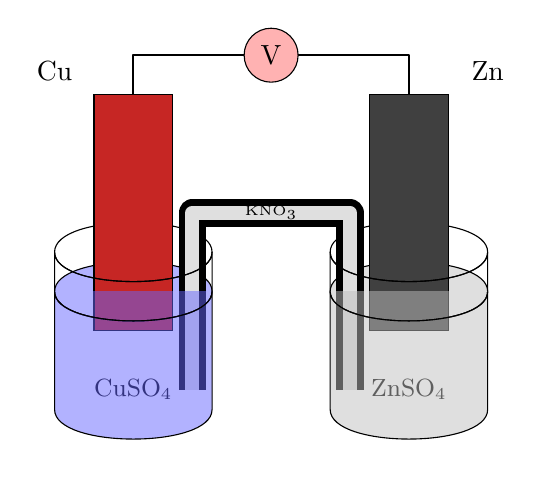
\begin{tikzpicture}
    % Draw back of vessel 1
    \draw (0,0) to [controls=+(90:0.5) and +(90:0.5)] (2,0);
    \draw[fill=blue!60, fill opacity=0.5] (0,-0.5) to
        [controls=+(90:0.5) and +(90:0.5)] (2,-0.5);

    % Draw back of vessel 2
    \draw (3.5,0) to [controls=+(90:0.5) and +(90:0.5)] (5.5,0);
    \draw[fill=lightgray, fill opacity=0.5] (3.5,-0.5) to [controls=+(90:0.5)
        and +(90:0.5)] (5.5,-0.5);

    % Draw copper electrode
    \draw[fill=copper] (0.5,2) rectangle (1.5,-1);
    \draw (0,2.3) node {Cu};
    \draw (1,-1.75) node {\small{CuSO$_{4}$}};

    % Draw salt bridge

    \draw[join=round, line width = 10pt] (1.75,-1.75) -- (1.75,0.5) --
        (3.75, 0.5) -- (3.75,-1.75);
    \draw[join=round, line width = 5pt, color = gray!25] (1.75,-1.75) --
        (1.75,0.5) -- (3.75, 0.5) -- (3.75,-1.75);
    \draw (2.75,0.5) node {\tiny{KNO$_{3}$}};

    %Draw front of vessel 1

    \draw (0,0) .. controls +(-90:0.5) and +(-90:0.5) .. (2,0);
    \draw (0,0) .. controls +(-90:0.5) and +(-90:0.5) .. (2,0)
        -- (2,-0.5) .. controls +(-90:0.5) and +(-90:0.5) .. (0,-0.5) -- (0,0);

    %Second part

    \draw[fill=blue!60, fill opacity=0.5] (0,-0.5) .. controls +(-90:0.5)
    and +(-90:0.5) .. (2,-0.5);
    \draw[fill=blue!60, fill opacity=0.5] (0,-0.5) .. controls +(-90:0.5)
    and +(-90:0.5) .. (2,-0.5)
        -- (2,-2) .. controls +(-90:0.5) and +(-90:0.5) .. (0,-2) -- (0,-0.5);

    % draw voltmeter

    \draw[join = round, thick] (1,2) -- (1,2.5) -- (4.5,2.5) -- (4.5,2);
    \draw (2.75,2.5) node [circle, draw, fill=red!30] {V};

    %Draw back of vessel 2

    %Draw electrode

    \draw[fill=darkgray] (4,2) rectangle (5,-1);
    \draw (5.5,2.3) node {Zn};
    \draw (4.5,-1.75) node {\small{ZnSO$_{4}$}};

    % Draw front of vessel 2
    % part 1
    \draw (3.5,0) .. controls +(-90:0.5) and +(-90:0.5) .. (5.5,0);
    \draw (3.5,0) .. controls +(-90:0.5) and +(-90:0.5) .. (5.5,0)
        -- (5.5,-0.5) .. controls +(-90:0.5) and +(-90:0.5)
        .. (3.5,-0.5) -- (3.5,0);
    % part 2
    \draw[fill=lightgray, fill opacity=0.5] (3.5,-0.5) .. controls +(-90:0.5)
    and +(-90:0.5) .. (5.5,-0.5);
    \draw[fill=lightgray, fill opacity=0.5] (3.5,-0.5) .. controls +(-90:0.5)
        and +(-90:0.5) .. (5.5,-0.5) --
        (5.5,-2) .. controls +(-90:0.5) and +(-90:0.5)
        .. (3.5,-2) -- (3.5,-0.5);

\end{tikzpicture}
\end{center}
\end{wrapfigure}
La pile Daniell est constituée de deux compartiments liés par un pont salin.
\begin{itemize}
	\item Le premier compartiment se compose d'une plaque de cuivre \\plongée dans une solution de sulfate de cuivre $(Cu^{2+} + SO_4^{2-})$, \\ce qui constitue la 1ère demi-pile qu'on appelle \textbf{électrode.}

	\item Le deuxième compartiment se compose d'une plaque de \\zinc plongée dans une solution de sulfate de zinc \\$(Zn^{2+}+SO_4^{2-})$, c'est l'autre demi-pile qu'on appelle aussi \textbf{électrode.}

	\item Le pont salin (ou ionique) qui relie les deux solutions il est constitué d'une solution de chlorure de potassium $(K^+ + Cl^-)$ qui est un conducteur électrolytique.

	\item On a ainsi réalisé une pile électrochimique.
\end{itemize}

\subsubsection{Fonctionnement de la pile Daniell : }

Un ampèremètre branché aux bornes de la pile indique le passage du courant électrique de la plaque de cuivre vers la plaque
de zinc. (Les électrons circulent alors dans ce circuit extérieur de la plaque de zinc vers la plaque de cuivre).
\begin{itemize}
	\item La plaque de cuivre qui représente le pôle positif de la pile s'appelle: \textbf{la cathode.}
\item La plaque de zinc qui représente le pôle négatif de la pile s'appelle \textbf{l'anode.}

\end{itemize}


\subsubsection{Réaction aux électrodes: }

Au cours du fontionnement de la pile: 

\begin{itemize}

	\item La masse de l'électrode de zinc diminue, elle se consomme, ceci est due à l'oxydation du zinc selon la demi-équation: $\ce{Zn <=> Zn^{2+} + 2e^-}$  \textbf{	--oxydation anodique --}

	\item La masse de l'électrode de cuivre augmente, ceci est due à la réduction des ions $Cu^{2+}$ en cuivre selon la demi-équation: $\ce{Cu^{2+}  + 2e^- <=> Cu}$  \textbf{-- réduction cathodiquue -- }

	\item L'équation globale de la réaction qui se produit pendant le fonctionnement de la pile s'obtient en ajoutant les deux demi équations précédentes. $$\ce{Cu^{2+}_{(aq)}  + Zn_{(s)} <=>[1][2] Cu_{(s)} + Zn^{2+}_{(aq)}}$$

	\item La constante d'équilibre associée à cette réaction est: $K=1,9.10^{37}$ et $Q_{r,i} = \frac{[Zn^{2+}]_i}{[Cu^{2+}]_i} = 1 < K$
	\item Le critère d’évolution spontanée montre que l'équilibre évolue spontanément dans le sens (1) , c'est-à-dire le sens direct .
Donc la pile lorsqu’elle débite, elle constitue un système hors équilibre.
\end{itemize}


\subsubsection{Rôle du pont salin: }

Le pont salin a deux rôles: 

\begin{itemize}
	\item il permet la \textbf{liaison électrique} entre les deux compartiments sans que les deux solutions se mélangent, par migration des
conducteurs ioniques.

\item il assure la \textbf{neutralité électrique }des deux solutions.

(Car pendant le fonctionnement de la pile la concentration des ions $Zn^{2+}$ augmente dans la solution de sulfate de zinc et celle
des ions $Cu^{2+}$ diminue dans la solution de sulfate de cuivre et pour assurer la neutralité électrique les ions $Cl^-$ migrent à travers
le pont ionique vers la solution de sulfate de zinc et les ions $K^+$ vers la solution de sulfate de cuivre).
\end{itemize}

\subsubsection{Représentation conventionnelle de la pile:}

On représente symboliquement la pile Daniell par la représentation conventionnelle suivante: 

\begin{center}
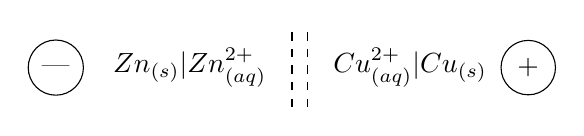
\begin{tikzpicture}

	
\node[circle,draw] (c) at (0,0){---};
\node[] at(1.7,0) {$Zn_{(s)}|Zn^{2+}_{(aq)}$};

\draw[dashed] (3,-0.5) -- (3,0.5);
\draw[dashed] (3.2,-0.5) -- (3.2,0.5);
\node[] at(4.5,0) {$Cu^{2+}_{(aq)} | Cu_{(s)}$};
\node[circle,draw] (c) at (6,0){+};
\end{tikzpicture}

\end{center}

\subsection{Généralisation :}
On peut réaliser des piles identiques à la pile Daniell.
En général une pile est constituée :
\begin{itemize}
	\item D'une plaque d'un métal M plongé dans une solution contenant les ions métalliques $M^{m+}$ de ce métal.
	\item D'une plaque d'un autre métal N plongé dans une solution contenant les ions métalliques $N^{n+}$ de ce métal.
\item D'un pont salin qui relie les deux solutions.
\item représentation conventionnelle : 
\begin{center}
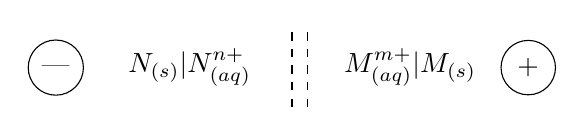
\begin{tikzpicture}

	
\node[circle,draw] (c) at (0,0){---};
\node[] at(1.7,0) {$N_{(s)}|N^{n+}_{(aq)}$};

\draw[dashed] (3,-0.5) -- (3,0.5);
\draw[dashed] (3.2,-0.5) -- (3.2,0.5);
\node[] at(4.5,0) {$M^{m+}_{(aq)} | M_{(s)}$};
\node[circle,draw] (c) at (6,0){+};
\end{tikzpicture}

\end{center}

\item l'anode :     $\ce{N <=> N^{n+} + ne^-}$  \textbf{	--oxydation anodique --}
\item la cathode :  $\ce{M^{m+}  + me^- <=> M}$  \textbf{-- réduction cathodiquue -- }

	\item L'équation globale de la réaction qui se produit pendant le fonctionnement de la pile s'obtient en ajoutant les deux demi équations précédentes. $$\ce{nM^{m+}_{(aq)}  + mN_{(s)} <=>[1][2] nM_{(s)} + mN^{n+}_{(aq)}}$$

	\item La pile électrochimique convertit l'énergie chimique (résultant d'un transfert spontané d'électrons entre deux couples oxydant -
réducteur) en énergie électrique

\end{itemize}

\begin{center}

	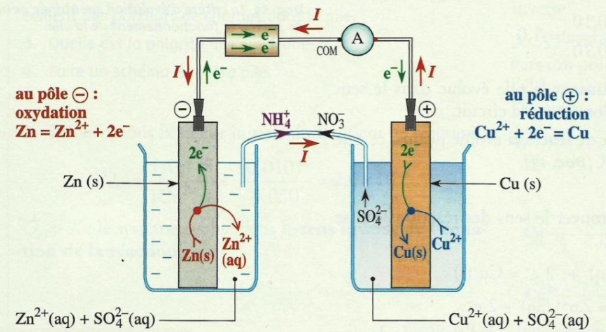
\includegraphics[width=0.5\textwidth]{./piles.png}

\end{center}


\section{Détermination de la polarité d'une pile: }

Pour déterminer expérimentalement la polarité d'une pile on utilise l'une des deux méthodes suivantes:

\section*{1-ère méthode:}
On branche un ampèremètre entre les bornes de la pile.
\begin{itemize}
	\item  Si Celui ci indique une intensité du courant électrique positive, alors sa borne COM est donc liée au pôle négatif de la pile.
	\item  Et s'il indique une intensité du courant électrique négative, sa borne COM est liée au pôle positif de la pile.
\end{itemize}


\section*{2-ème méthode:}

Connaissant les deux couples d'oxydoréduction qui interviennent dans la pile et la constante d'équilibre on utilise le critère
d'évolution pour trouver le sens de la réaction spontanée qui se produit dans la pile ce qui permettra de savoir l'électrode à
laquelle se produit l'oxydation qui est l'anode (pôle négatif ) et l'autre c'est la cathode (pôle positif )de la pile.


\subsection{Exercice d'application de la 1ère méthode: }

On réalise la pile suivante:


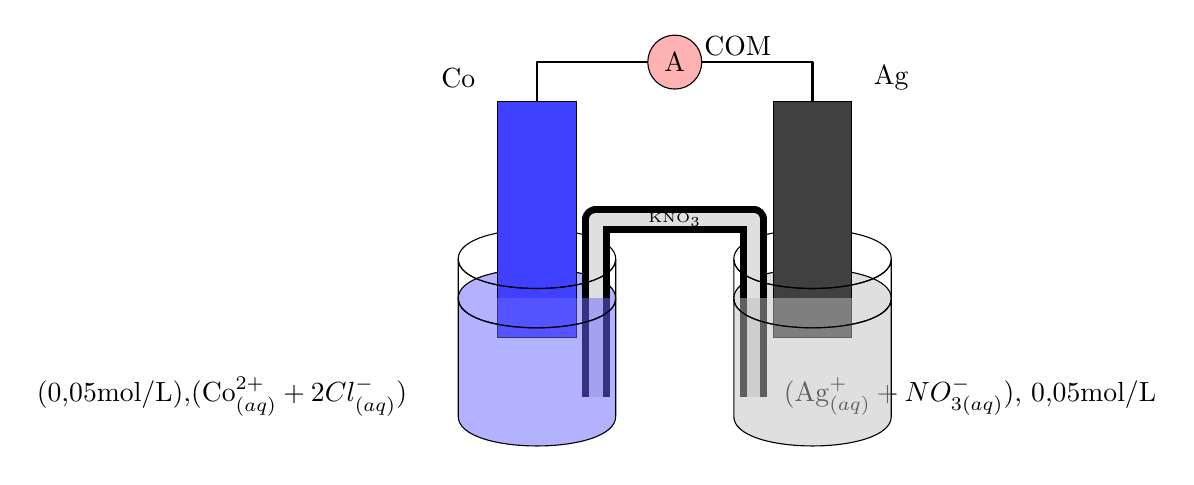
\begin{tikzpicture}
    % Draw back of vessel 1
    \draw (0,0) to [controls=+(90:0.5) and +(90:0.5)] (2,0);
    \draw[fill=blue!60, fill opacity=0.5] (0,-0.5) to
        [controls=+(90:0.5) and +(90:0.5)] (2,-0.5);

    % Draw back of vessel 2
    \draw (3.5,0) to [controls=+(90:0.5) and +(90:0.5)] (5.5,0);
    \draw[fill=lightgray, fill opacity=0.5] (3.5,-0.5) to [controls=+(90:0.5)
        and +(90:0.5)] (5.5,-0.5);

    % Draw copper electrode
    \draw[fill=blue!75] (0.5,2) rectangle (1.5,-1);
    \draw (0,2.3) node {Co};
\draw (-3,-1.75) node {(0,05mol/L),(Co$^{2+}_{(aq)} +2Cl^-_{(aq)}$)};

    % Draw salt bridge

    \draw[join=round, line width = 10pt] (1.75,-1.75) -- (1.75,0.5) --
        (3.75, 0.5) -- (3.75,-1.75);
    \draw[join=round, line width = 5pt, color = gray!25] (1.75,-1.75) --
        (1.75,0.5) -- (3.75, 0.5) -- (3.75,-1.75);
    \draw (2.75,0.5) node {\tiny{KNO$_{3}$}};

    %Draw front of vessel 1

    \draw (0,0) .. controls +(-90:0.5) and +(-90:0.5) .. (2,0);
    \draw (0,0) .. controls +(-90:0.5) and +(-90:0.5) .. (2,0)
        -- (2,-0.5) .. controls +(-90:0.5) and +(-90:0.5) .. (0,-0.5) -- (0,0);

    %Second part

    \draw[fill=blue!60, fill opacity=0.5] (0,-0.5) .. controls +(-90:0.5)
    and +(-90:0.5) .. (2,-0.5);
    \draw[fill=blue!60, fill opacity=0.5] (0,-0.5) .. controls +(-90:0.5)
    and +(-90:0.5) .. (2,-0.5)
        -- (2,-2) .. controls +(-90:0.5) and +(-90:0.5) .. (0,-2) -- (0,-0.5);

    % draw voltmeter

    \draw[join = round, thick] (1,2) -- (1,2.5) -- (4.5,2.5) -- (4.5,2);
    \draw (2.75,2.5) node [circle, draw, fill=red!30] {A};
    \draw (3.55,2.7) node [] {COM};

    %Draw back of vessel 2

    %Draw electrode

    \draw[fill=darkgray] (4,2) rectangle (5,-1);
    \draw (5.5,2.3) node {Ag};
	\draw (6.5,-1.75) node {{(Ag$^+_{(aq)} + NO_{3(aq)}^-$), 0,05mol/L}};

    % Draw front of vessel 2
    % part 1
    \draw (3.5,0) .. controls +(-90:0.5) and +(-90:0.5) .. (5.5,0);
    \draw (3.5,0) .. controls +(-90:0.5) and +(-90:0.5) .. (5.5,0)
        -- (5.5,-0.5) .. controls +(-90:0.5) and +(-90:0.5)
        .. (3.5,-0.5) -- (3.5,0);
    % part 2
    \draw[fill=lightgray, fill opacity=0.5] (3.5,-0.5) .. controls +(-90:0.5)
    and +(-90:0.5) .. (5.5,-0.5);
    \draw[fill=lightgray, fill opacity=0.5] (3.5,-0.5) .. controls +(-90:0.5)
        and +(-90:0.5) .. (5.5,-0.5) --
        (5.5,-2) .. controls +(-90:0.5) and +(-90:0.5)
        .. (3.5,-2) -- (3.5,-0.5);

\end{tikzpicture}



Sachant que l'ampèremètre indique une intensité négative.

1) Déterminer la polarité de cette pile puis donner sa représentation symbolique conventionnelle.

2) Ecrire l'équation de la demi-réaction qui se produit près de chaque électrode puis en déduire l'équation globale de
la réaction qui se produit lors du fonctionnement de la pile.

3) Quel est le rôle du pont salin?

4) Calculer le quotient initial de cette réaction.

5) Comment évolue ce quotient de la réaction durant le fonctionnement de la pile?



\section*{Exercice d'application de la deuxième méthode: }

On lie avec un pont salin les deux demi-piles suivantes:
\begin{itemize}
	\item  Une électrode de cuivre Cu plongée dans une solution de sulfate de cuivre $(Cu^{2+}+SO_4^{2-})$, $[Cu^{2+}]_i=0,05mol/L$.

	\item Une électrode d'argent Ag plongée dans une solution de sulfate d'argent $(Ag^++NO_{3-})$, $[Ag^+]_i=0,01mol/L$.
\end{itemize}

Sachant que la constante d'équilibre associée à la réaction suivante :$$\ce{2Ag_{(s)} + Cu^{2+}_{aq} <=>[1][2] 2Ag^+_{(aq)} + Cu_{(s)}  }$$ est $K =2,6 10^{-16}$

1) Déterminer le sens d'évolution spontanée de cet équilibre puis en déduire l'équation globale de la réaction qui se produit
durant le fonctionnement de la pile.

2) Ecrire l'équation de la demi-réaction qui se produit près de chaque électrode puis en déduire la polarité de la pile.

3) Donner la représentation symbolique conventionnelle de la pile.


\section{Quantité d'électricité maximale débitée par une pile: }

La quantité d'électricité qui traverse le conducteur liant les deux bornes d'une pile durant le temps $\Delta{t}$ est : $q=I.\Delta{t}$

D'autre part: $q = N.e$ car les porteurs de charge sont les électrons :

n: est le nombre des électrons qui traversent le conducteur pendant le temps $\Delta{t}$ .

donc :$$N.e = I.\Delta{t}$$ d’où: $$N = \frac{I.\Delta{t}}{e}$$

La quantité de matière des électrons correspondant est : $n(e)= \frac{N}{N_A}$ 

$N_A$: nombre d'Avogadro. Donc: $n(e) = \frac{I.\Delta{t}}{N_A.e}$

La grandeur :$F=N_A.e$ s'appelle le faraday (Le faraday est la valeur absolue de la charge d'une mole d'électrons)

Donc la quantité de matière des électrons qui traversent le conducteur pendant le temps $\Delta{t}$.$$n(e)=\frac{I.\Delta{t}}{F}$$

$F = 6,02.10^{23}.1,6.10^{-19}  = 96500C/mol$

\begin{tcolorbox}
Remarque: Si la pile débite un courant d'intensité I pendant un temps $\Delta{t}$: 
avant d'être usée, elle délivre une quantité d'électricité $Q_{max} = I.\Delta{t}$ 

avec $Q_{max} :$ représente la capacité en charge de la pile (c'est la quantité d'électricité maximale qu'elle peut débiter avant d'être usée)



\end{tcolorbox}


\section*{Exercice d'application: }

On considère une pile dont la représentation conventionnelle est : 
\begin{center}
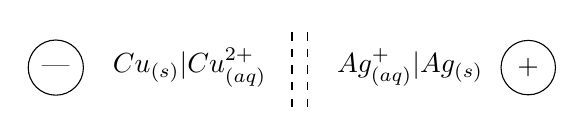
\begin{tikzpicture}

	
\node[circle,draw] (c) at (0,0){---};
\node[] at(1.7,0) {$Cu_{(s)}|Cu^{2+}_{(aq)}$};

\draw[dashed] (3,-0.5) -- (3,0.5);
\draw[dashed] (3.2,-0.5) -- (3.2,0.5);
\node[] at(4.5,0) {$Ag^{+}_{(aq)} | Ag_{(s)}$};
\node[circle,draw] (c) at (6,0){+};
\end{tikzpicture}

\end{center}
L'équation de la réaction d'oxydoréduction qui se produit pendant le fonctionnement de la pile est:

$\ce{2Ag^+_{(aq)} + Cu_{(s)} <=> 2Ag_{(s)} + Cu^{2+}_{(aq)}}$

Sachant que la pile débite pendant un temps $\Delta{t} = 1,5mn$
un courant d'intensité $I=86mA$.

1) Quelle est la quantité d'électricité transportée pendant ce temps?

2) Dresser le tableau d'avancement de cette réaction puis déterminer l'expression de l'avancement x en fonction de I,$\Delta{t}$ et F et  calculer sa valeur.

3) Déterminer la variation de la masse de chaque électrode pendant le temps $\Delta{t}$.

4) Déterminer la variation quantité de matière des ions $Cu^{2+}$ et celle des ions Ag+ dans la pile pendant le temps $\Delta{t}$.

On donne : F = 96500C/mol , M(Ag) = 108g/mol , M(Cu) = 63,5g/mol

%\begin{figure}[h!]
	%\begin{center}
	%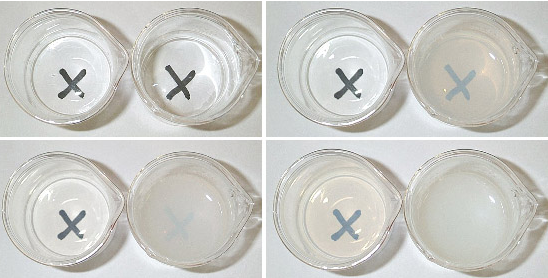
\includegraphics[width=0.5\textwidth]{./img/TRLconcentration.png}
%\end{center}
%\vspace{-1cm}
%\end{figure}



%\begin{wrapfigure}[10]{r}{0.5\textwidth}
%    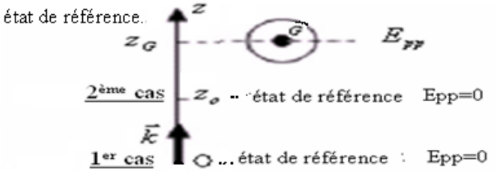
\includegraphics[width=0.5\textwidth]{./img/img00.png}
%\end{wrapfigure}


%\begin{center}
   %\begin{tabular}{|c|c|c|}
      %\hline
      %Indicateur coloré & Couleur de l’espèce acide & Couleur de l’espèce base\\\hline
      %BBT               & Jaune                     & Bleue\\\hline
      %Hélianthine       &Rose                       & Jaune\\\hline
      %Phénolphtaléine   & inclore                   & rose \\\hline
   %\end{tabular}
%\end{center}

\end{document}

